\documentclass {article}
\usepackage[utf8]{inputenc}
\usepackage{amsmath}
\usepackage{graphicx}
\usepackage{soul}
\begin{document}

\section{Solve graphically}
Find two positive numbers that minimize the sum of twice the first number plus second if product of two is 288.\\
\\
- Assume that the first and second numbers are $a$ and $b$, respectively.\\
- Using the given information, we already know:\\ 

\begin{align*}
	a > 0 \\
	b > 0 \\
	ab = 288 \\
	b=\frac{288}{a} \\
	f(x)= 2a + b \\
	f(x)= 2a + \frac{288}{a} \\
\end{align*}

and we need to find out the number $a$ that minimizes the function:\\

\begin{align*}
	f(x)= 2a + \frac{288}{a} \\
\end{align*}

\begin{figure}
  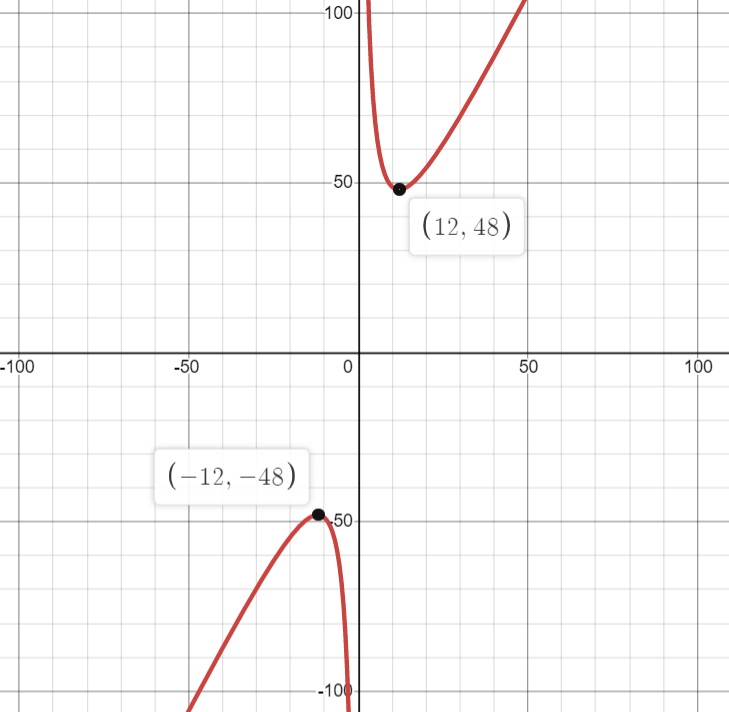
\includegraphics[width=\linewidth]{graph1.png}
  \caption{Graph of $f(x)= 2a + \frac{288}{a}$}
\end{figure}

We can tell from the below graph that f(x) has a local minimum of $(12,48)$ and since $a > 0$ in this case, it is also the global minimum of $f(x)$.

\begin{align*}
a = 12 \\
\\
b = \frac{288}{a} \\
\\
b = \frac{288}{12} \\
\\
b = 24 \\
\end{align*}

The two positive numbers the minimize the sum of twice the first number plus the second number if the product of the two is 288 is: $a = 12, b = 24$\\
ANSWER: $a = 12, b = 24$

\section{Solve algebraically}
Find two positive numbers whose product is 750 and for which the sum of one and 10 times the other is a minimum.\\
\\
- Assume that the first and second numbers are $a$ and $b$, respectively.\\
- Using the given information, we already know:\\ 

\begin{align*}
	a > 0 \\
	b > 0 \\
	ab = 750 \\
	b=\frac{750}{a} \\
	f(x)= a+10b \\
	f(x)= a+\frac{7500}{a}\\
\end{align*}
\\
To algebraically determine the minimum in this case, we have to find which point on the function does its tangent line have a slope of zero. Although this sounds fairly complicated, this point is found by finding the derivative of the function and setting it equal to zero since the derivative $\frac{d}{dx}$ represents rate of change at any given point and we're looking for a slope of zero at a particular point.\\
\\

\begin{align*}
	f(a)=a + 7500a^{-1}\\
	\frac{d}{da}f(a)=\frac{d}{da}(a) + 7500*\frac{d}{da}(a^{-1})\\
	\frac{d}{da}f(a)=1+7500*(-a^{-2})\\
	\frac{d}{da}f(a)=1+\frac{-7500}{a^2}\\
	\frac{d}{da}f(a)=0\\
	1+\frac{-7500}{a^2}=0\\
	\frac{-7500}{a^2}=-1\\
	-7500=(-a)^2\\
	a=50\sqrt{3}\\
	a=-50\sqrt{3} [rejected]\\
	\\
	b=\frac{750}{50\sqrt{3}}\\
	b=5\sqrt{3}
\end{align*}

The answer to the question, "What two positive numbers whose product is 750 and for which the sum of one and 10 times the other is a minimum?" is: $a=50\sqrt{3}, b=5\sqrt{3}$.


\end{document}